\section{Polynomier}
Vi betragtede tidligere første- og andengradsligninger, hvor venstre siden var på formen $ax+b$ og $ax^2+bx+c$, henholdsvis. Dette er to eksempler på funktionstyper som man kalder polynomier. Disse funktioner vil vi nu studere mere dybdegående. 

\paragraph*{Førstegradspolynomier:}
En funktion med forskrift
\begin{align*}
f(x)=ax+b,
\end{align*}
hvor $a \in \mathbb{R}\setminus \{0\}$ og $b \in \mathbb{R}$, kaldes for et førstegradspolynomium. I genkender formentlig et førstegradspolynomium som ligningen for en ret linje.
\begin{figure}[!htbp]
  \centering
  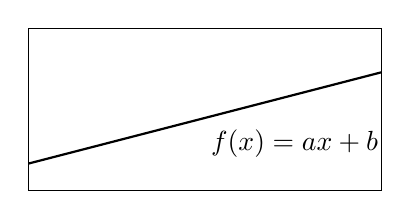
\begin{tikzpicture}
  \begin{axis}[ 
  	width=0.5\textwidth,
  	height=0.3\textwidth,
    xmin=-0.1,
    xmax=3,
    ymin=-0.1,
    ymax=1,
    %axis equal,
    %axis lines=center,
	ticks=none,
	restrict y to domain =0:1]
	\addplot[thick] {0.2*x+0.1} node[below right,pos=0.4] {$f(x)=ax+b$};
\end{axis}
 \end{tikzpicture}
  \caption{Førstegradspolynomium.}
  \label{fig:funktioner3et}
\end{figure}

Hvis vi sætter $x=0$ i vores førstegradspolynomium får vi at 
\begin{align*}
f(0)=a\cdot 0 + b = b,
\end{align*}
hvilket viser at et førstegradspolynomium skærer $y$-aksen i $b$. Derudover får vi, hvis vi indsætter $x+1$ på $x$ plads at
\begin{align*}
f(x+1)=a(x+1)+b = a + (ax+b)=a+f(x),
\end{align*}
hvilket viser at hvis vi går $1$ ud ad $x$-aksen, så gå vi $a$ op ad $y$-aksen og vi kalder derfor $a$ for hældningen af vores rette linje.

Hvis man får givet to punkter $(x_1,y_1)$ og $(x_2,y_2)$ i et koordinatsystem, så kan man bestemme forskriften for den rette linje der går gennem de to punkter ud fra formlerne
\begin{align*}
a= \frac{y_2-y_1}{x_2-x_1} \qquad \textup{ og } \qquad b= f(x_1)-ax_1 = y_1 - ax_1.
\end{align*}
Bemærk, at man også kan bruge punktet $(x_2,y_2)$ til at finde $b$.

\paragraph*{Eksempler:}
\begin{enumerate}
\item Givet punkterne $P=(1,7)$ og $Q=(2,4)$, bestem en forskrift for $f$:

Vi udregner først $a$:
\begin{align*}
a= \frac{y_2-y_1}{x_2-x_1} = \frac{4-7}{2-1}=\frac{-3}{1}=-3.
\end{align*}
Det bruger vi så sammen med punktet $P$ til at bestemme $b$:
\begin{align*}
b=y_1 - ax_1=7- (-3) \cdot 1 = 10, 
\end{align*}
hvilket giver at forskriften for $f$ er givet ved $f(x)=-3x+10$.
\item Lad funktionerne $f$ og $g$ være givet ved henholdsvis $f(x)=-x+2$ og $g(x)=2x+2$ og find det punkt hvor de skærer hinanden.

Vi vil finde den værdi for $x$ der gør at $f(x)=g(x)$. Det gør vi ved at sætte de to forskrifter lig med hinanden og så isolere $x$:
\begin{align*}
f(x)=g(x) &\Leftrightarrow -x+2 = 2x+2 \\
&\Leftrightarrow -3x = 0 \\
&\Leftrightarrow x = 0.
\end{align*}
Ved at indsætte $x=0$ i forskriften for enten $f$ eller $g$ får vi at $y=2$, hvilket viser at $f$ og $g$ skærer hinanden i punktet $(0,2)$.
\end{enumerate}

\paragraph*{Andengradspolynomier:}
En funktion med forskrift
\begin{align*}
f(x)=ax^2+bx+c,
\end{align*}
hvor $a \in \mathbb{R} \setminus \{0\}$ og $b,c \in \mathbb{R}$, kaldes for et andengradspolynomium. Grafen for et andengradspolynomium er en parabel (se Figur~\ref{fig:funktioner3to}).
\begin{figure}[!htbp]
  \centering
  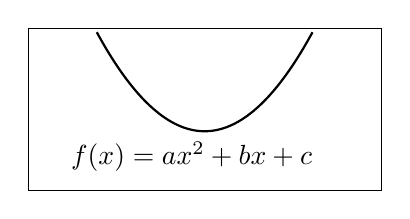
\begin{tikzpicture}
  \begin{axis}[ 
  	width=0.5\textwidth,
  	height=0.3\textwidth,
    xmin=-3,
    xmax=3,
    ymin=-0.1,
    ymax=1,
%    axis equal,
%    axis lines=center,
	ticks=none,
	restrict y to domain =0:1]
	\addplot[thick,samples=200] {0.2*x^2+0.2+0.1} node[below,pos=0.5] {$f(x)=ax^2+bx+c \phantom{ss}$};
\end{axis}
 \end{tikzpicture}
  \caption{Andengradspolynomium.}
  \label{fig:funktioner3to}
\end{figure}

Ved at sætte $x=0$ får vi, at et andengradspolynomium skærer $y$-aksen i
\begin{align*}
f(0)=a\cdot 0^2 + b \cdot 0 + c = c.
\end{align*}
Hvis vi differentierer $f(x)$, får vi
\begin{align*}
f'(x)=2ax+b,
\end{align*}
og ved igen at indsætte $x=0$ får vi at $f'(0)=b$. Vi husker at den afledte funktion beskriver hældningen i punktet, hvilket medfører, at $b$ beskriver hvad hældningen af vores andengradspolynomium er i skæringspunktet med $y$-aksen.

Til sidst ser vi, at hvis $x$ bliver meget stor, så bliver $x^2$ meget større end $x$ gør. Det betyder, at leddet $ax^2$ bestemmer om $f(x)$ går mod $+ \infty$ eller $-\infty$ når $x$ bliver meget stor. Da $x^2$ altid er positiv, har vi, at fortegnet på $a$ bestemmer om vores parabel går opad eller nedad. 

Hvis man får givet tre punkter $(x_1,y_1)$, $(x_2,y_2)$ og $(x_3,y_3)$, kan man entydigt bestemme det andengradspolynomium der går gennem de punkter ved at løse de tre ligninger med tre ubekendte:
\begin{align*}
f(x_1)&=ax_1^2+bx_1+c = y_1, \\
f(x_2)&=ax_2^2+bx_2+c = y_2, \\
f(x_3)&=ax_3^2+bx_2+c = y_3.
\end{align*}

\paragraph*{Toppunktsformlen:}
Hvis $a > 0$ i vores andengradspolynomium så kaldes det punkt med den mindste funktionsværdi for andengradspolynomiets toppunkt og hvis $a < 0$ så kaldes punktet med den største funktionsværdi for toppunktet. Vi notere toppunktet med $(x_0,y_0)$, hvor $x_0$ og $y_0$ kan bestemmes ud fra formlerne
\begin{align*}
x_0 = \frac{-b}{2a} \qquad \textup{ og } \qquad y_0=\frac{-d}{4a},
\end{align*}
hvor vi husker at $d=b^2-4ac$.


\paragraph*{Eksempler:}
\begin{enumerate}
\item Lad $f(x)= 2x^2+2x-2$ og bestem funktionens toppunkt.

Vi ser at $a=2$, $b=2$ og $c=-2$, hvilket medfører at $d=2^2-4 \cdot 2 \cdot (-2)=20$. Indsætter vi dette i formlerne for toppunktet får vi
\begin{align*}
x_0 = \frac{-2}{4} = \frac{-1}{2} \qquad \textup{ og } \qquad y_0 = \frac{-20}{8}=\frac{-5}{2},
\end{align*}
hvilket giver at toppunktet er $\big(\frac{-1}{2},\frac{-5}{2}\big)$.
\item Givet de tre punkter $(-1,1)$, $(0,1)$ og $(-2,-2)$, bestem en ligning for det dertilhørende andengradspolynomium.

Vi har de tre ligninger
\begin{align*}
a(-1)^2+b(-1) + c = 1 &\Leftrightarrow a-b+c=1,\\
a(0)^2+b(0) + c = 1 &\Leftrightarrow c=1,\\
a(-2)^2+b(-2) + c = -2 &\Leftrightarrow 4a-2b +c = -2.
\end{align*}
Fra ligning to ser vi at $c=1$ og ved at indsætte dette i de to andre, får vi to ligninger med to ubekendte:
\begin{align*}
a-b+1=1 &\Leftrightarrow a-b=0, \\
4a-2b+1=-2 &\Leftrightarrow 4a-2b = -3.
\end{align*}
Hvis vi benytter de lige store koefficienters metode til at løse disse to ligninger, får vi at
\begin{align*}
4a-2b = -3 &\Leftrightarrow 4a - 2b -4(a-b) = -3 \\
&\Leftrightarrow 2b = -3 \\
&\Leftrightarrow b = \frac{-3}{2}.
\end{align*}
Indsætter vi nu dette i ligningen $a-b=0$ får vi at $a=\frac{-3}{2}$, så vores andengradspolynomium er:
\begin{align*}
f(x)=-\frac{3}{2}x^2 -\frac{3}{2}x+1.
\end{align*}
\end{enumerate}












